% !TeX program = lualatex -synctex=1 -interaction=nonstopmode --shell-escape %.tex
\documentclass[_Banking_p2.tex]{subfiles}
\begin{document}

\setbeamercovered{invisible}
\subsection{Системы оценки кредитоспособности}
\begin{frame}[shrink=15]{Системы оценки кредитоспособности}
% Table generated by Excel2\textsl{•}LaTeX from sheet 'Лист2'
\begin{table}[htbp]
\caption{Наиболее распространенные системы оценки кредитоспособности клиента}
  \centering
  	\begin{tabularx}{\linewidth}[b]{@{}>{\raggedright\arraybackslash}XX@{}}
    \toprule
    \multicolumn{1}{>{\centering\arraybackslash}m{30mm}}{«Правило пяти си» (США)} & \multicolumn{1}{>{\centering\arraybackslash}m{40mm}}{CAMPARI (некоторые европейские банки)} \\
    \midrule
    \textbf{C} – character (репутация заемщика) 

    \textbf{C} – capacity (финансовые возможности) 

    \textbf{C} – capital (капитал, имущество) 

    \textbf{C} – collateral (обеспечение) 

    \textbf{C} – conditions (общие экономические условия)  

    & 

    \textbf{C} – character (репутация заемщика)

    \textbf{A} – ability (способность возвратить кредит)
    
    \textbf{M} – marge (доходность кредитной операции)
    
    \textbf{P} – purpose (целевое назначение кредита)
    
    \textbf{A} – amount (размер кредита)
    
    \textbf{R} – repayment (условия погашения)
    
    \textbf{I} – insurance (обеспечение)\\
    \bottomrule
    \end{tabularx}%
  \label{tab:addlabel}%
\end{table}%

\end{frame}

\begin{frame}[shrink=20]{}

% Table generated by Excel2LaTeX from sheet 'Лист2'
\begin{table}[htbp]
\caption{Наиболее распространенные системы оценки кредитоспособности клиента}
  \centering
  	\begin{tabularx}{\linewidth}[b]{@{}>{\raggedright\arraybackslash}XXX@{}}
    \toprule
    \multicolumn{1}{>{\centering\arraybackslash}m{35mm}}{COPF
    
     (Германия)} & \multicolumn{1}{>{\centering\arraybackslash}m{40mm}}{CAMEL 
    
    (Мировой банк)
}
    & \multicolumn{1}{>{\centering\arraybackslash}m{35mm}}{PARSER
    
     (Англия)
} \\
    \midrule
    C – competition (конкуренция в отрасли)

	O – organization (организация деятельности)

	P – personnel (персонал, кадры)

	F – finance (финансы, доходы)

    & 
	C – capital (достаточность собственного капитала)

	A – assets (размер активов)

	M – management (качество менеджмента)

	E – earning (доходность)

	L – liquidity (ликвидность)

	&
	
	P – person (репутация заемщика)

	A – amount (сумма кредита)

	R – repayment (возможности погашения)

	S – security (обеспечение)

	E – expediency (целесообразность кредита)

	R – remuneration (вознаграждение банку)
\\
    \bottomrule
    \end{tabularx}%
  \label{tab:addlabel}%
\end{table}%

\end{frame}

\begin{frame}[ allowframebreaks ]{Симптомы возможной финансовой опасности для банка }
\begin{itemize}
\item
налаживание предприятием производства ранее не выпускавшейся продукции и освоение в связи с этим нового рынка сбыта;
\item
появление зависимости клиента от кредитов (обычно краткосрочных) в связи с увеличивающимися накладными расходами;
\item
упущения клиента в контроле над своим оборотным капиталом (общий избыток товарных запасов и т.д.);

\pagebreak
\item
наличие у клиента крупных и непредвиденных потерь;
\item
нарушение клиентом сроков подготовки отчетности или представления в банк необходимых финансовых документов;
\item
просьбы клиента о выделении ему дополнительных средств, сверх ранее согласованных лимитов;
\item
любое немотивированное несоблюдение обязательств.
\end{itemize}
\end{frame}

\begin{frame}[ allowframebreaks ]{Признаки надвигающегося финансового кризиса заемщика}
\begin{itemize}
\item
значительное превышение согласованных лимитов;
\item
нецелевое расходование средств полученного кредита;
\item
скудные и нерегулярные поступления денег от реализации товаров, особенно в сочетании со значительными выплатами поставщикам и неоправданным ростом продаж в кредит;

\pagebreak
\item
выплаты другим кредитным организациям или резкое увеличение числа запросов от них о финансовом состоянии клиента;
\item
манипуляции клиента с чеками.
\end{itemize}
\end{frame}

\subsection{Кредитный скоринг}
\subsubsection{Финансовые коэффициенты}
\begin{frame}{Финансовый анализ кредитоспособности предприятий}{}
Методы скоринга:
\begin{align}
P=\sum_i{k_i\cdot X_i}
\end{align}

Где

\textit{P} – общая оценка финансового положения предприятия в баллах, определяющая риск банкротства; чем выше оценка, тем меньше риск.

$X_i$ – показатели (как правило, получены на основе финансовой отчетности предприятия).

$k_i$ – коэффициенты, заранее присваиваемые каждому из показателей.
\end{frame}

\begin{frame}[ allowframebreaks ]{Классификация финансовых коэффициентов}

\textbf{Коэффициенты ликвидности}:

- коэффициент текущей ликвидности (коэффициент покрытия);

- коэффициент оперативной ликвидности;

\bigskip
\textbf{Коэффициенты эффективности (оборачиваемости)}:

- коэффициент оборачиваемости дебиторской задолженности;

- коэффициент оборачиваемости запасов товарно-материальных ценностей;

- коэффициент оборачиваемости основных средств;

- коэффициент оборачиваемости активов

\pagebreak
\textbf{Коэффициенты финансового левериджа }(зависимости от внешних источников) рассчитываются в отношении активов, капитала, уставного капитала и т.д.

\bigskip
Коэффициенты прибыльности:

- коэффициенты доходности;

- коэффициенты рентабельности;

- коэффициенты прибыльности акций.

\bigskip
\textbf{Коэффициенты обслуживания долгов} рассчитываются в виде отношения общей прибыли заемщика к тем или иным предстоящим ему платежам.

\pagebreak
\textbf{В дополнение }финансовое положение заемщика оценивается на основе:

- анализа денежных потоков;

- анализа делового риска (возможность того, что предприятие не сможет достигнуть заявленных целей).


\end{frame}

\begin{frame}{Примеры оценки кредитоспособности}
{Публичное акционерное общество ``СОЛЛЕРС''}
ОАО ``СОЛЛЕРС'' - российская автомобильная компания, которая занимается производством машин, а также их продажей и сервисным обслуживанием. В структуру компании входят: ОАО ``Ульяновский автомобильный завод'', ОАО ``Заволжский моторный завод'', ОАО ``Соллерс-Набережные Челны'', ООО ``Соллерс-Елабуга'', ООО ``Соллерс-Дальний Восток''. 

54\% акций находится в свободном обращении.
\end{frame}

\begin{frame}{}
\begin{figure}	
\centering
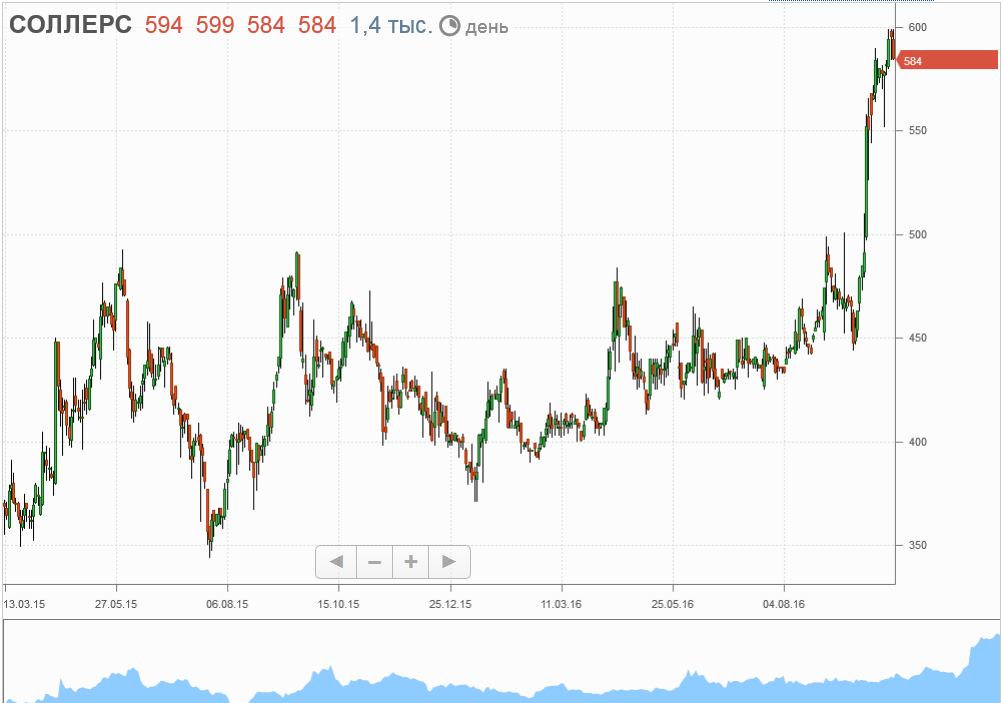
\includegraphics[scale=0.3]{img/SVAV_quotes.png}
\caption{Котировки акций ``СОЛЛЕРС''\\ 
Источник: АО ``Инвестиционная компания ФИНАМ'', \url{http://www.finam.ru}.}\label{fig:SVAV_quotes}
\end{figure}
\end{frame}

\begin{frame}{Примеры оценки кредитоспособности}
{Открытое акционерное общество ``Авиационная компания Трансаэро''}
``Трансаэро'' – первая частная авиакомпания в России. Основана в 1990 г. Базируется в Москве и Санкт-Петербурге. 

\textbf{Определением Арбитражного суда }города Санкт-Петербурга и Ленинградской области от 16 декабря 2015 года (Резолютивная часть определения) по делу № А56-75891/2015 в отношении Открытого акционерного общества ``Авиационная компания ТРАНСАЭРО'' \textbf{введена процедура наблюдения}.
\end{frame}

\begin{frame}{}
\begin{figure}	
\centering
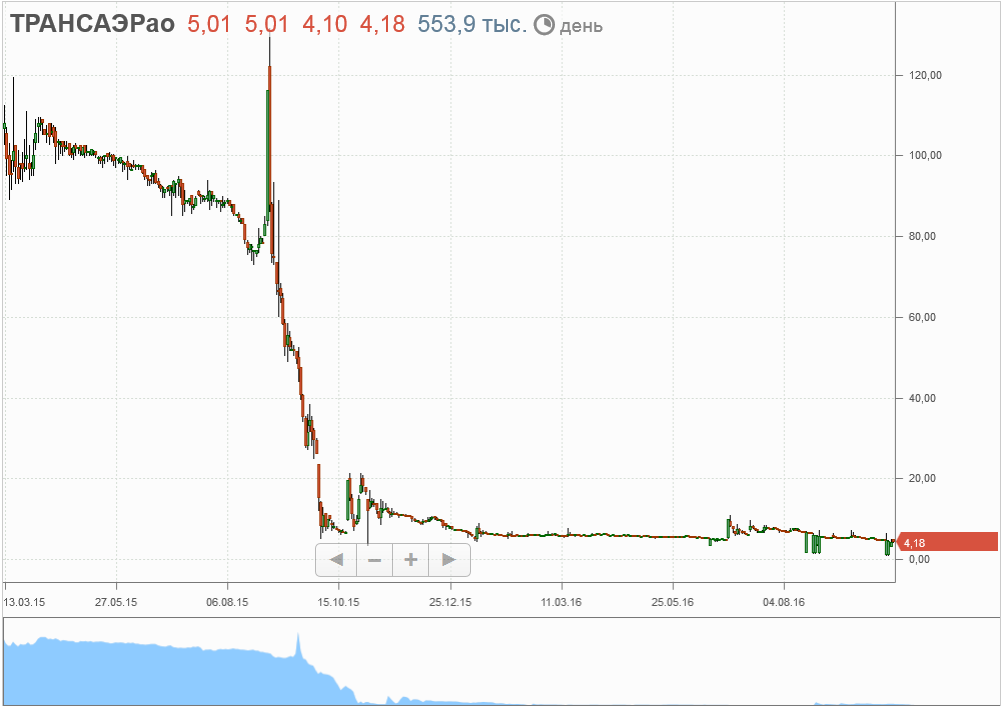
\includegraphics[scale=0.3]{img/TAER_quotes.png}
\caption{Котировки акций ``ТРАНСАЭРО''\\ 
Источник: АО ``Инвестиционная компания ФИНАМ'', \url{http://www.finam.ru}.}\label{fig:TAER_quotes}
\end{figure}

\end{frame}

\begin{frame}{Примеры оценки кредитоспособности}
{ Публичное акционерное общество ``Уралкалий''}
Объединенная компания ``Уралкалий'' создана в 2011 году путем присоединения ОАО ``Сильвинит'' к ОАО ``Уралкалий''. ``Уралкалий'' занимает первое место в мире по объемам производства хлористого калия. ``Уралкалий'' владеет ``Балтийским балкерным терминалом'' (Санкт-Петербург) и собственным парком железнодорожных вагонов. 

В свободном обращении находятся 33,26\% акций компании.
\end{frame}

\begin{frame}{}
\begin{figure}	
\centering
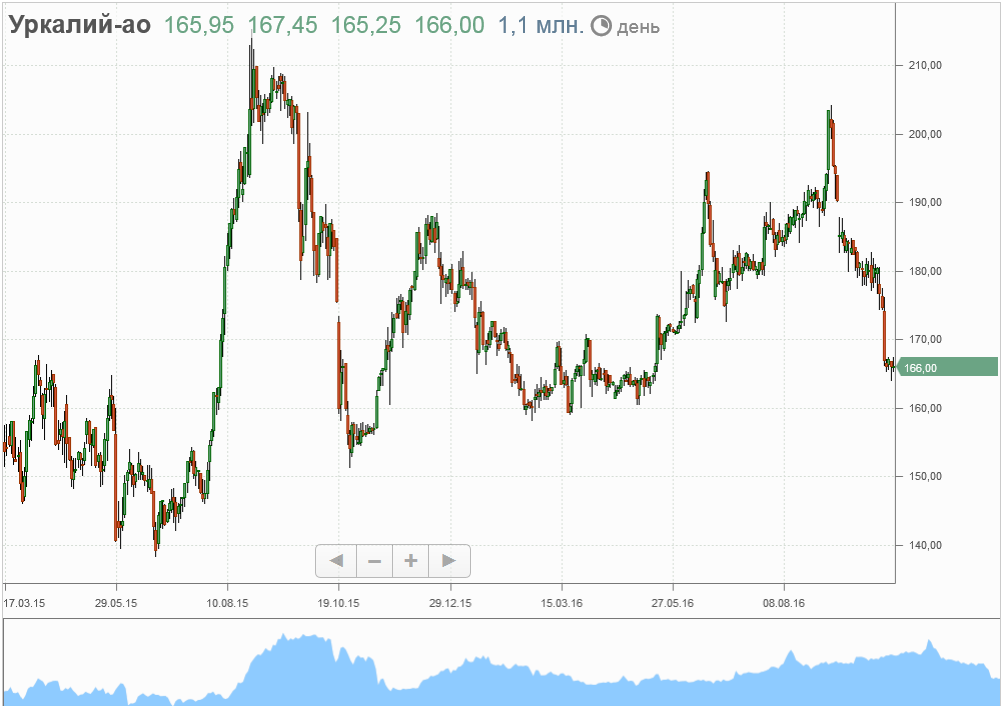
\includegraphics[scale=0.3]{img/URKA_quotes.png}
\caption{Котировки акций ``Уралкалий''\\ 
Источник: АО ``Инвестиционная компания ФИНАМ'', \url{http://www.finam.ru}.}\label{fig:URKA_quotes}
\end{figure}
\end{frame}

\begin{frame}[shrink=70]{Финансовая отчетность компаний Трансаэро, СОЛЛЕРС, Уралкалий}{Бухгалтерский баланс РСБУ (тыс. руб.)}
% Table generated by Excel2LaTeX from sheet 'Отчетность'
\begin{table}[htbp]
\caption{Бухгалтерский баланс РСБУ компаний Трансаэро, СОЛЛЕРС, Уралкалий (тыс. руб.)}
\centering
\begin{tabular}{L{8cm} lrrrrrr}
\toprule
\multirow{2}[0]{*}{Название показателя} & \multirow{2}[0]{*}{Сокр. об.} & \multicolumn{2}{c}{Трансаэро} & \multicolumn{2}{c}{СОЛЛЕРС} & \multicolumn{2}{c}{Уралкалий} \\\cline{3-8}
&       & \textbf{2Q15} & \textbf{2014} & \textbf{3Q15} & \textbf{2014} & \textbf{2Q16} & \textbf{2015} \\
\midrule
АКТИВ &       & \textbf{} & \textbf{} & \textbf{} & \textbf{} & \textbf{} & \textbf{} \\
I. Внеоборотные активы &       & \textbf{} & \textbf{} & \textbf{} & \textbf{} & \textbf{} & \textbf{} \\
Нематериальные активы & НМА   & 68 253 456 & 61 207 880 & 451   & 2 970 & 35 156 346 & 35 167 972 \\
Результаты исследований и разработок & НИОКР & 0     & 0     & 0     & 0     & 138 850 & 247 240 \\
Основные средства & ОС    & 17 099 607 & 12 658 216 & 93 295 & 97 769 & 108 139 989 & 99 150 384 \\
Доходные вложения в материальные ценности & ВМЦ   & 0     & 0     & 0     & 0     & 306 824 & 316 946 \\
Финансовые вложения & ДФВ   & 1 811 964 & 1 619 356 & 10 446 722 & 10 310 485 & 375 829 266 & 337 402 527 \\
Отложенные налоговые активы & ОНАф1 & 457 449 & 452 388 & 287 051 & 210 622 & 532 304 & 417 545 \\
Прочие внеоборотные активы & прВА  & 34 628 083 & 31 928 539 & 0     & 0     & 4 360 908 & 2 884 615 \\
Итог по разделу I & ВА    & 122 250 559 & 107 866 379 & 10 827 519 & 10 621 846 & 524 464 487 & 475 587 229 \\
II. Оборотные активы &       & \textbf{} & \textbf{} & \textbf{} & \textbf{} & \textbf{} & \textbf{} \\
Запасы & Зап   & 5 651 182 & 5 188 360 & 35    & 3 550 & 5 902 781 & 5 842 646 \\
Налог на добавленную стоимость по приобретённым ценностям & НДС   & 386 510 & 732 808 & 83    & 4     & 1 173 202 & 2 277 540 \\
Дебиторская задолженность & ДЗ    & 9 392 884 & 11 729 796 & 299 727 & 179 916 & 44 603 062 & 56 053 029 \\
Финансовые вложения & КФВ   & 3 585 450 & 2 959 269 & 881 500 & 970 500 & 2 211 955 & 0 \\
Денежные средства & ДС    & 988 664 & 360 560 & 107 616 & 709 360 & 71 438 577 & 62 838 126 \\
Прочие оборотные активы & прОА  & 25 396 & 25 395 & 3 246 & 29 677 & 435   & 2 365 \\
Итог по разделу II & ОА    & 20 030 086 & 20 996 188 & 1 292 207 & 1 893 007 & 125 330 012 & 127 013 706 \\
БАЛАНС & ВБ    & 142 280 645 & 128 862 567 & 12 119 726 & 12 514 853 & 649 794 499 & 602 600 935 \\
ПАССИВ &       & \textbf{} & \textbf{} & \textbf{} & \textbf{} & \textbf{} & \textbf{} \\
III. Капиталы и резервы &       & \textbf{} & \textbf{} & \textbf{} & \textbf{} & \textbf{} & \textbf{} \\
Уставной капитал (складочный капитал, уставной капитал, вклады товарищей) & УК    & 1 538 & 1 538 & 428 377 & 428 377 & 1 468 008 & 1 468 008 \\
Собственные акции выкупленные у акционеров & СобАкц & 0     & 0     & 0     & 0     & 0     & 0 \\
Переоценка внеоборотных активов & перВА & 73 435 642 & 66 389 268 & 0     & 0     & 4 178 461 & 4 239 053 \\
Добавочный капитал (без переоценки) & ДобКап & 0     & 0     & 3 167 527 & 3 167 527 & 0     & 0 \\
Резервный капитал & РезКап & 231   & 231   & 21 419 & 21 419 & 220 201 & 220 201 \\
Нераспределённая прибыль (непокрытый убыток) & НерПр & -60 263 460 & -51 677 292 & 3 998 282 & 3 601 247 & 141 922 291 & 96 700 673 \\
Итог по разделу III & СК    & 13 173 951 & 14 713 745 & 7 615 605 & 7 218 570 & 147 788 961 & 102 627 935 \\
IV. Долгосрочные обязательства &       & \textbf{} & \textbf{} & \textbf{} & \textbf{} & \textbf{} & \textbf{} \\
Заемные средства & ЗС    & 21 682 175 & 29 229 749 & 0     & 0     & 402 321 224 & 420 841 512 \\
Отложенные налоговые обязательства & ОНО   & 253 301 & 265 091 & 0     & 0     & 9 832 305 & 8 837 263 \\
Резервы под условные обязательства & резУО & 0     & 0     & 0     & 0     & 4 646 618 & 2 556 702 \\
Прочие обязательства & прО   & 0     & 0     & 0     & 0     & 0     & 0 \\
Итог по разделу IV & ДП    & 21 935 476 & 29 494 840 & 0     & 0     & 416 800 147 & 432 235 477 \\
V. Краткосрочные обязательства &       & \textbf{} & \textbf{} & \textbf{} & \textbf{} & \textbf{} & \textbf{} \\
Заемные средства & КЗаймы & 45 816 743 & 36 494 028 & 4 433 096 & 5 036 518 & 77 460 862 & 57 923 599 \\
Кредиторская задолженность & КЗ    & 61 038 407 & 47 832 060 & 56 541 & 153 763 & 6 275 101 & 8 608 984 \\
Доходы будущих периодов & ДБП   & 0     & 0     & 0     & 0     & 4 208 & 3 168 \\
Резервы предстоящих расходов & РПР   & 316 068 & 327 893 & 14 484 & 106 002 & 1 465 220 & 1 201 772 \\
Прочие обязательства & прКП  & 0     & 0     & 0     & 0     & 0     & 0 \\
Итог по разделу V & КП    & 107 171 218 & 84 653 981 & 4 504 121 & 5 296 283 & 85 205 391 & 67 737 523 \\
БАЛАНС & ВБ    & 142 280 645 & 128 862 566 & 12 119 726 & 12 514 853 & 649 794 499 & 602 600 935 \\
\bottomrule
\end{tabular}%
\label{tab:addlabel}%
\end{table}%
Источник: \href{http://investfunds.ru/}{Информационный ресурс Investfunds Группа Cbonds}

\end{frame}
\begin{frame}[shrink=70]{Финансовая отчетность компаний Трансаэро, СОЛЛЕРС, Уралкалий}{Отчёт о финансовых результатах РСБУ (тыс. руб.), по кварталам - нарастающим итогом}
% Table generated by Excel2LaTeX from sheet 'Отчетность'
\begin{table}[htbp]
\caption{Отчёт о финансовых результатах РСБУ компаний Трансаэро, СОЛЛЕРС, Уралкалий (тыс. руб.), по кварталам - нарастающим итогом}
\centering
\begin{tabular}{L{8cm}lrrrrrr}
\toprule
\multirow{2}[0]{*}{Название показателя} & \multirow{2}[0]{*}{Сокр. об.} & \multicolumn{2}{c}{Трансаэро} & \multicolumn{2}{c}{СОЛЛЕРС} & \multicolumn{2}{c}{Уралкалий} \\\cline{3-8}
&       & \textbf{2Q15} & \textbf{2014} & \textbf{3Q15} & \textbf{2014} & \textbf{2Q16} & \textbf{2015} \\
\midrule
Выручка & Вр    & 50 420 054 & 117 313 131 & 576 080 & 1 930 744 & 70 658 359 & 172 129 828 \\
Себестоимость продаж & Сс    & -50 432 881 & -109 451 785 & -550 068 & -1 674 628 & -16 312 314 & -30 971 641 \\
Валовая прибыль (убыток) & ВП    & -12 826 & 7 861 346 & 26 012 & 256 116 & 54 346 045 & 141 158 187 \\
Коммерческие расходы & КомРасх & -2 501 997 & -3 063 158 & 0     & 0     & -11 617 365 & -23 838 487 \\
Управленческие расходы & УпрРасх & -2 457 747 & -5 091 528 & -244 001 & -17 606 & -4 691 069 & -8 941 207 \\
Прибыль (убыток) от продаж & ПП    & -4 972 571 & -293 339 & -217 989 & 238 510 & 38 037 611 & 108 378 493 \\
Доходы от участия в других организациях & ДивПолуч & 15 184 & 27 530 & 762 888 & 2 865 308 & 898 000 & 2 262 996 \\
Проценты к получению & ПроцПолуч & 219 315 & 344 389 & 94 157 & 44 528 & 374 309 & 6 004 779 \\
Проценты к уплате & ПроцУпл & -6 432 412 & -7 827 105 & -564 165 & -373 500 & -10 656 540 & -16 932 970 \\
Прочие доходы & прД   & 8 843 905 & 4 261 328 & 416 618 & 568 542 & 42 305 548 & 3 128 257 \\
Прочие расходы & прР   & -6 169 732 & -16 071 305 & -170 904 & -392 745 & -16 218 149 & -67 696 854 \\
Прибыль (убыток) до налогообложения & ПДН   & -8 496 311 & -19 558 501 & 320 605 & 2 950 643 & 54 740 779 & 35 144 701 \\
Текущий налог на прибыль & НП    & 0     & 0     & 0     & 0     & -8 668 686 & -2 166 451 \\
- в т.ч. постоянные налоговые обязательства (активы) & постНА & -1 682 412 & -3 612 360 & -140 551 & -636 578 & -89 696 & 307 001 \\
Изменение отложенных налоговых обязательств & измНО & 11 790 & -35 860 & 155   & -333  & -446 307 & -492 991 \\
Изменение отложенных налоговых активов & измНА & 5 060 & 335 200 & 76 275 & 46 783 & 102 550 & -2 486 759 \\
Прочее & прДох & -97 138 & -63 308 & 0     & 0     & -567 310 & 284 579 \\
Чистая прибыль (убыток) & ЧП    & -8 576 599 & -19 322 469 & 397 035 & 2 997 093 & 45 161 026 & 30 283 079 \\
СПРАВОЧНО &       & \textbf{} & \textbf{} & \textbf{} & \textbf{} & \textbf{} & \textbf{} \\
Результат по переоценке внеоборотных активов, не включаемый в чистую прибыль (убыток) &       & 0     & 63 972 855 & 0     & 0     & 0     & 0 \\
Результат от прочих операций, не включаемых в чистую прибыль (убыток) периода &       & 0     & 0     & 0     & -1 795 013 & 0     & 0 \\
Совокупный финансовый результат периода &       & -8 576 599 & 44 650 386 & 397 035 & 1 202 080 & 45 161 026 & 30 283 079 \\
Базовая прибыль (убыток) на акцию & ПрАкц & 0     & 0     & 0     & 0     & 0     & 10 \\
Разводненная прибыль (убыток) на акцию & развПрАкц & 0     & 0     & 0     & 0     & 0     & 0 \\
Источник: http://stocks.investfunds.ru &       &       &       &       &       &       &  \\
СПРАВОЧНО (доп.) &       &       &       &       &       &       &  \\
Дивиденды, тыс. руб. & Див   & 0     & 0     & 0     & 0     & 0     & 0 \\
Коэффициент реинвестирования & кРеинв & 1,000 & 1,000 & 1,000 & 1,000 & 1,000 & 1,000 \\
Кол-во акций в обращении, шт. &       & 153 755 868 & 153 755 868 & 34 270 159 & 34 270 159 & 2 936 018 072 & 2 936 018 072 \\
Цена акции &       & 92    & 103   & 439   & 370   & 176   & 151 \\
Капитализация & Кап   & 14 145 540 & 15 836 854 & 15 044 600 & 12 679 959 & 516 739 181 & 443 338 729 \\
\bottomrule
\end{tabular}%
\label{tab:addlabel}%
\end{table}%
Источник: \href{http://investfunds.ru/}{Информационный ресурс Investfunds Группа Cbonds}
\end{frame}
\subsubsection{Альтман}
\begin{frame}[shrink=25]{Модель Альтмана}{}
Для компаний на развитых рынках, акции которых котируются на бирже:
\begin{align}
Z=1,2 \cdot x_1+1.4\cdot x_2+3.3\cdot x_3+0,6\cdot x_4+0.999\cdot x_5	
\end{align}
Для частных компаний:		
\begin{align}
Z=0,717\cdot x_1 &+0,847\cdot x_2+3,107\cdot x_3\nonumber \\ &+0,42\cdot x_4+0.995\cdot x_5
\end{align}
где				

$x_1$ — отношение оборотного капитала к сумме активов;

$x_2$ — отношение резервов к сумме активов;

$x_3$ — отношение операционной прибыли к сумме активов;

$x_4$ — отношение рыночной стоимости акций к задолженности (для компаний, акции которых котируются на бирже) или отношение балансовой стоимости собственных средств к привлеченным средствам (для компаний, акции которых не котируются на бирже);

$x_5$ — отношение выручки к сумме активов.
Справка: Альтман - профессор финансов Нью-Йоркского университета.
\end{frame}

\begin{frame}{Критерии кредитоспособности по Альтману}
\textbf{Для компаний,\linebreak акции которых котируются на бирже:
}

< 1,8 — предприятия являются безусловно-несостоятельными;

1,81-2,99 — зона неопределенности;

> 3,0 — финансово устойчивые предприятия.
\end{frame}

\begin{frame}{Критерии кредитоспособности по Альтману}
\textbf{Для компаний, \linebreak акции которых не котируются на бирже:
}

< 1,23 — предприятия являются безусловно-несостоятельными;

1,23-2,90 — зона неопределенности;

> 2,90 — финансово устойчивые предприятия.

\bigskip
\end{frame}

\begin{frame}[shrink=20]{Модель Альтмана}{Трансаэро}
% Table generated by Excel2LaTeX from sheet 'Альтман'
\begin{table}[htbp]
\centering
\small
\caption{\captionf{Для развитых рынков}}
\begin{tabularx}{\linewidth}[b]{@{}>{\raggedright\arraybackslash}Xcrrcrr@{}}
\setrulecolor\toprule &                     & \multicolumn{2}{c}{\cnamef{$k_i$}} &  & \multicolumn{2}{c}{\cnamef{Трансаэро}} \\
\rules{3-4}{6-7}      &                     & \cnamef{бирж.} & \cnamef{част.}    &  & \cnamef{2Q15} & \cnamef{2014}          \\ \midrule
x1                    & (ОА-КП) / ВБ        & 1,20           & 0,72              &  & -0,61         & -0,49                  \\
x2                    & (РезКап+НерПр) / ВБ & 1,40           & 0,85              &  & -0,42         & -0,40                  \\
x3                    & (ПДН+ПроцУп) / ВБ   & 3,30           & 3,11              &  & -0,10         & -0,21                  \\
x4                    & Кап / (ДП+КП)       & 0,60           & 0,42              &  & 0,11          & 0,14                   \\
x5                    & Вр / ВБ             & 1,00           & 1,00              &  & 0,35          & 0,91                   \\ \midrule
Z                     & $\sum(k_i * x_i)$   & 2,68           &                   &  & -1,25         & -0,86                  \\
& Биржевая            &                &                   &  & Да            & Да                     \\ \midrule
& Вывод               &                &                   &  & банкр.        & банкр.                 \\ \bottomrule
\end{tabularx}%
\label{tab:addlabel}%
\end{table}%
\end{frame}




\iftagged{professor}
{
\begin{frame}[shrink=20]{Модель Альтмана}{СОЛЛЕРС}

% Table generated by Excel2LaTeX from sheet 'Альтман'
\begin{table}[htbp]
\centering
\small
\caption{\captionf{Для развитых рынков}}
\begin{tabularx}{\linewidth}[b]{@{}>{\raggedright\arraybackslash}Xcrrcrr@{}}
\setrulecolor\toprule &                     & \multicolumn{2}{c}{\cnamef{$k_i$}} &  & \multicolumn{2}{c}{\cnamef{СОЛЛЕРС}} \\
\rules{3-4}{6-7}      &                     & \cnamef{бирж.} & \cnamef{част.}    &  & \cnamef{3Q15} & \cnamef{2014}          \\ \midrule
	x1 & (ОА-КП) / ВБ        & 1,20 & 0,72 &  & \onslide<2->{-0,27 } & \onslide<2->{-0,27} \\
	x2 & (РезКап+НерПр) / ВБ & 1,40 & 0,85 &  & \onslide<3->{0,33  } & \onslide<3->{0,29 } \\
	x3 & (ПДН+ПроцУп) / ВБ   & 3,30 & 3,11 &  & \onslide<4->{-0,02 } & \onslide<4->{0,21 } \\
	x4 & Кап / (ДП+КП)       & 0,60 & 0,42 &  & \onslide<5->{3,34  } & \onslide<5->{2,39 } \\
	x5 & Вр / ВБ             & 1,00 & 1,00 &  & \onslide<6->{0,05  } & \onslide<6->{0,15 } \\ \midrule
	Z  & $\sum(k_i * x_i)$   & 2,68 &      &  & \onslide<7->{2,13  } & \onslide<7->{2,35 } \\
	   & Биржевая            &      &      &  & \onslide<8->{Да    } & \onslide<8->{Да   } \\ \midrule
	   & Вывод               &      &      &  & \onslide<9->{неопр.} & \onslide<9->{неоп } \\ \bottomrule
\end{tabularx}%
\label{tab:addlabel}%
\end{table}%
\end{frame}

\begin{frame}[shrink=20]{Модель Альтмана}{Уралкалий}

% Table generated by Excel2LaTeX from sheet 'Альтман'
\begin{table}[htbp]
\centering
\small
\caption{\captionf{Для развитых рынков}}
\begin{tabularx}{\linewidth}[b]{@{}>{\raggedright\arraybackslash}Xcrrcrr@{}}
\setrulecolor\toprule &                     & \multicolumn{2}{c}{\cnamef{$k_i$}} &  & \multicolumn{2}{c}{\cnamef{Уралкалий}} \\
\rules{3-4}{6-7}      &                     & \cnamef{бирж.} & \cnamef{част.}    &  & \cnamef{2Q16} & \cnamef{2015}          \\ \midrule
	x1 & (ОА-КП) / ВБ        & 1,20 & 0,72 &  & \onslide<2->{0,06  } & \onslide<2->{0,10  } \\
	x2 & (РезКап+НерПр) / ВБ & 1,40 & 0,85 &  & \onslide<3->{0,22  } & \onslide<3->{0,16  } \\
	x3 & (ПДН+ПроцУп) / ВБ   & 3,30 & 3,11 &  & \onslide<4->{0,07  } & \onslide<4->{0,03  } \\
	x4 & Кап / (ДП+КП)       & 0,60 & 0,42 &  & \onslide<5->{1,03  } & \onslide<5->{0,89  } \\
	x5 & Вр / ВБ             & 1,00 & 1,00 &  & \onslide<6->{0,11  } & \onslide<6->{0,29  } \\ \midrule
	Z  & $\sum(k_i * x_i)$   & 2,68 &      &  & \onslide<7->{1,33  } & \onslide<7->{1,26  } \\
	   & Биржевая            &      &      &  & \onslide<8->{Да    } & \onslide<8->{Да    } \\ \midrule
	   & Вывод               &      &      &  & \onslide<9->{банкр.} & \onslide<9->{банкр.} \\ \bottomrule
\end{tabularx}%
\label{tab:addlabel}%
\end{table}%
\end{frame}

}

\begin{frame}[shrink=20]{Модель Альтмана}{Трансаэро}
% Table generated by Excel2LaTeX from sheet 'АльтманEM'
\begin{table}[htbp]
\centering
\caption{\captionf{Для развивающихся рынков}}
\begin{tabularx}{\linewidth}[b]{@{}>{\raggedright\arraybackslash}Xccrr@{}}
	\setrulecolor\toprule &                       &                &   \multicolumn{2}{c}{\cnamef{Трансаэро}}    \\
	\cmidrule{4-5}        &                       & \cnamef{$k_i$} & \cnamef{2Q15}        & \cnamef{2014}        \\ \midrule
	x1                    & (ОА - КП) / ВБ        & 6,560          & \onslide<2->{-0,612} & \onslide<2->{-0,494} \\
	x2                    & ПП / ВБ               & 3,260          & \onslide<3->{-0,035} & \onslide<3->{-0,002} \\
	x3                    & ПДН / ВБ              & 6,720          & \onslide<4->{-0,060} & \onslide<4->{-0,152} \\
	x4                    & СК / (ДП + КП)        & 1,050          & \onslide<5->{0,102 } & \onslide<5->{0,129 } \\
	$Z_{EM}$              & $\sum(k_i \cdot x_i)$ & -              & \onslide<6->{-4,426} & \onslide<6->{-4,133} \\ \midrule
	Вывод:                &                       &                & \onslide<7->{банкр.} & \onslide<7->{банкр.} \\ \bottomrule
\end{tabularx}%
\label{tab:addlabel}%
\end{table}%
\end{frame}

\begin{frame}[shrink=20]{Модель Альтмана}
{Определение кредитного рейтинга заемщика для развивающегося рынка}
% Table generated by Excel2LaTeX from sheet 'АльтманEM'
\begin{table}[htbp]
\caption{Определение кредитного рейтинга Трансаэро}
\centering
\begin{tabular}{cccc}
\toprule
ЭР США & $Z_{EM}$ & ЭР США & РР балл \\
\midrule
ААА   & 8,15  & ВВ+   & 5,25 \\
АА+   & 7,6   & ВВ    & 4,95 \\
АА    & 7,3   & ВВ-   & 4,75 \\
АА-   & 7     & В+    & 4,5 \\
А+    & 6,85  & В     & 4,15 \\
А     & 6,65  & В-    & 3,75 \\
А-    & 6,4   & ССС+  & 3,2 \\
ВВВ+  & 6,25  & CCC   & 2,5 \\
ВВВ   & 5,85  & CCC-  & 1,75 \\
ВВВ-  & 5,65  & D     & 0 \\
\bottomrule
\end{tabular}%
\label{tab:addlabel}%
\end{table}%
ЭР США - эквивалентный рейтинг по облигациям эмитентов США;

$Z_{EM}$ - значение кредитного рейтинга по модели Альтмана для развивающихся рынков.
\end{frame}

\begin{frame}{Модель Альтмана\\ для развивающихся рынков}
{Корректировка рейтинга}
% Table generated by Excel2LaTeX from sheet 'АльтманEM'
\begin{table}[htbp]
\centering
\caption{Корректировка рейтинга на волатильность валютного рынка}
\begin{tabular}{lr}
\toprule
Волатильность & Изменения в рейтинге \\
\midrule
Высокая & минус 1 класс \\
Нейтральная & минус 1 отметка \\
Низкая & без изменений \\
\bottomrule
\end{tabular}%
\label{tab:addlabel}%
\end{table}%

Корректировка рейтинга на отраслевой риск:

от -1 до 2 отметок

\end{frame}

\begin{frame}{Модель Альтмана\\ для развивающихся рынков}
{Корректировка рейтинга}
% Table generated by Excel2LaTeX from sheet 'АльтманEM'
\begin{table}[htbp]
\centering
\caption{Корректировка рейтинга на конкурентную позицию компании в отрасли}
\begin{tabular}{lr}
\toprule
Позиция & Изменения в рейтинге \\
\midrule
Доминирующая & плюс 1 отметка \\
Средняя & без изменений \\
Слабая & минус 1 отметка \\
\bottomrule
\end{tabular}%
\label{tab:addlabel}%
\end{table}%

При определении доходности облигации эмитента с развивающегося рынка к полученной по данной методике величине нужно добавить спред суверенного дефолта между развивающейся страной и США	

\end{frame}

\iftagged{professor}{
\begin{frame}[shrink=20]{Модель Альтмана}{СОЛЛЕРС}
% Table generated by Excel2LaTeX from sheet 'АльтманEM'
\begin{table}[htbp]
\centering
\caption{\captionf{Для развивающихся рынков}}
\begin{tabularx}{\linewidth}[b]{@{}>{\raggedright\arraybackslash}Xccrr@{}}
\setrulecolor\toprule &                       &                & \multicolumn{2}{c}{\cnamef{СОЛЛЕРС}} \\
\cmidrule{4-5}        &                       & \cnamef{$k_i$} & \cnamef{3Q15} & \cnamef{2014}        \\ \midrule
	x1       & (ОА - КП) / ВБ        & 6,560 & \onslide<2->{-0,265} & \onslide<2->{-0,272} \\
	x2       & ПП / ВБ               & 3,260 & \onslide<3->{-0,018} & \onslide<3->{0,019 } \\
	x3       & ПДН / ВБ              & 6,720 & \onslide<4->{0,026 } & \onslide<4->{0,236 } \\
	x4       & СК / (ДП + КП)        & 1,050 & \onslide<5->{1,691 } & \onslide<5->{1,363 } \\
	$Z_{EM}$ & $\sum(k_i \cdot x_i)$ & -     & \onslide<6->{0,156 } & \onslide<6->{1,294 } \\ \midrule
	Вывод:   &                       &       & \onslide<7->{банкр.} & \onslide<7->{неопр.} \\ \bottomrule
\end{tabularx}%
\label{tab:addlabel}%
\end{table}%
\end{frame}

\begin{frame}[shrink=20]{Модель Альтмана}{Уралкалий}
% Table generated by Excel2LaTeX from sheet 'АльтманEM'
\begin{table}[htbp]
\centering
\caption{\captionf{Для развивающихся рынков}}
\begin{tabularx}{\linewidth}[b]{@{}>{\raggedright\arraybackslash}Xccrr@{}}
\setrulecolor\toprule &                       &                & \multicolumn{2}{c}{\cnamef{Уралкалий}} \\
\cmidrule{4-5}        &                       & \cnamef{$k_i$} & \cnamef{2Q16} & \cnamef{2015}          \\ \midrule
	x1       & (ОА - КП) / ВБ        & 6,560 & \onslide<2->{0,062 } & \onslide<2->{0,098 } \\
	x2       & ПП / ВБ               & 3,260 & \onslide<3->{0,059 } & \onslide<3->{0,180 } \\
	x3       & ПДН / ВБ              & 6,720 & \onslide<4->{0,084 } & \onslide<4->{0,058 } \\
	x4       & СК / (ДП + КП)        & 1,050 & \onslide<5->{0,294 } & \onslide<5->{0,205 } \\
	$Z_{EM}$ & $\sum(k_i \cdot x_i)$ & -     & \onslide<6->{1,471 } & \onslide<6->{1,839 } \\ \midrule
	Вывод:   &                       &       & \onslide<7->{неопр.} & \onslide<7->{неопр.} \\ \bottomrule
\end{tabularx}%
\label{tab:addlabel}%
\end{table}%
\end{frame}
}

\subsubsection{Чессер}
\begin{frame}{Статистическая модель Чессера\\ надзора за ссудами}{}
\begin{block}{Модель Чессера }
\quad – банковская методика оценки вероятности невыполнения заемщиком условий кредитного договора. Под невыполнением условий договора подразумевается не только невозврат суммы, но и любые другие отклонения от договора, делающие ссуду для кредитора менее выгодной.
\end{block}
\end{frame}
\begin{frame}[ allowframebreaks ]{Статистическая модель Чессера надзора за ссудами}
\begin{align}
Y = const + \sum_{i=1}^{6}X_i
\end{align}
Где 

X1 – (Денежные средства + Краткосрочные финансовые вложения) / Совокупные активы,

X2 – Выручка / (Денежные средства + Краткосрочные финансовые вложения),

X3 – Прибыль до налогообложения / Совокупные активы,

X4 – Совокупная задолженность / Совокупные активы,

X5 – Внеоборотные активы / Собственные средства,

X6 – Оборотные активы / Выручка;

const - Поправочный коэффициент.

\pagebreak
Формула для вероятности невыполнения условий договора
\begin{align}
P = \frac{1}{1 + e^{-Y}}, \text{где }  e = 2,71828
\end{align}
Модель определяет вероятность банкротства заемщика, значение вероятности ниже 50\% позволяет отнести заемщика к группе надежных.
\end{frame}

\begin{frame}[shrink=20]{Модель Чессера}{Трансаэро}
% Table generated by Excel2LaTeX from sheet 'Чессер'
\begin{table}[htbp]
\centering
\footnotesize
\caption{\captionf{Вероятность банкротства Трансаэро}}
\begin{tabularx}{\linewidth}[b]{@{}>{\raggedright\arraybackslash}cXrrr}
	\setrulecolor\toprule &                        &                &     \multicolumn{2}{c}{\cnamef{Трансаэро}}      \\
	\cmidrule{4-5}        &                        & \cnamef{$k_i$} & \cnamef{2Q15}          & \cnamef{2014}          \\ \midrule
	X1                    & (ДС + КФВ) / ВБ        & -5,240         & \onslide<2->{0,032 }   & \onslide<2->{0,026  }  \\
	X2                    & Вр / (ДС + КФВ)        & 0,005          & \onslide<3->{11,023}   & \onslide<3->{35,337 }  \\
	X3                    & ПДН / ВБ               & -6,651         & \onslide<4->{-0,060}   & \onslide<4->{-0,152 }  \\
	X4                    & (ДП + КП) / ВБ         & 4,401          & \onslide<5->{0,907 }   & \onslide<5->{0,886  }  \\
	X5                    & ВА / ОА                & -0,079         & \onslide<6->{6,103 }   & \onslide<6->{5,137  }  \\
	X6                    & ОА / Вр                & -0,122         & \onslide<7->{0,397 }   & \onslide<7->{0,179  }  \\
	Y                     & $k_Y + \sum (x_i*k_i)$ & -2,043         & \onslide<8->{1,706 }   & \onslide<8->{2,489  }  \\ \midrule
	P                     & $1 / (1 + e^{(-Y)})$   & 0,500          & \onslide<9->{0,846 }   & \onslide<9->{0,923  }  \\ \midrule
	Выводы:               &                        &                & \onslide<10->{некр-сп} & \onslide<10->{некр-сп} \\ \bottomrule
\end{tabularx}%
\label{tab:addlabel}%
\end{table}%
\end{frame}

\iftagged{professor}{
\begin{frame}[shrink=20]{Модель Чессера}{СОЛЛЕРС}
% Table generated by Excel2LaTeX from sheet 'Чессер'
\begin{table}[htbp]
\centering
\footnotesize
\caption{\captionf{Вероятность банкротства СОЛЛЕРС}}
\begin{tabularx}{\linewidth}[b]{@{}>{\raggedright\arraybackslash}cXrrr}
\setrulecolor\toprule &                        &                & \multicolumn{2}{c}{\cnamef{СОЛЛЕРС}} \\
\cmidrule{4-5}        &                        & \cnamef{$k_i$} & \cnamef{2Q15} & \cnamef{2014} \\ \midrule
	X1      & (ДС + КФВ) / ВБ        & -5,240 & \onslide<2 ->{0,082  } & \onslide<2 ->{0,134  } \\
	X2      & Вр / (ДС + КФВ)        & 0,005  & \onslide<3 ->{0,582  } & \onslide<3 ->{1,149  } \\
	X3      & ПДН / ВБ               & -6,651 & \onslide<4 ->{0,026  } & \onslide<4 ->{0,236  } \\
	X4      & (ДП + КП) / ВБ         & 4,401  & \onslide<5 ->{0,372  } & \onslide<5 ->{0,423  } \\
	X5      & ВА / ОА                & -0,079 & \onslide<6 ->{8,379  } & \onslide<6 ->{5,611  } \\
	X6      & ОА / Вр                & -0,122 & \onslide<7 ->{2,243  } & \onslide<7 ->{0,980  } \\
	Y       & $k_Y + \sum (x_i*k_i)$ & -2,043 & \onslide<8 ->{-1,945 } & \onslide<8 ->{-3,010 } \\ \midrule
	P       & $1 / (1 + e^{(-Y)})$   & 0,500  & \onslide<9 ->{0,125  } & \onslide<9 ->{0,047  } \\ \midrule
	Выводы: &                        &        & \onslide<10->{кред-сп} & \onslide<10->{кред-сп} \\ \bottomrule
\end{tabularx}%	кред-сп & кред-сп 
\label{tab:addlabel}%
\end{table}%
\end{frame}
\begin{frame}[shrink=20]{Модель Чессера}{Уралкалий}
% Table generated by Excel2LaTeX from sheet 'Чессер'
\begin{table}[htbp]
\centering
\footnotesize
\caption{\captionf{Вероятность банкротства Уралкалий}}
\begin{tabularx}{\linewidth}[b]{@{}>{\raggedright\arraybackslash}cXrrr}
	\setrulecolor\toprule &                        &                &     \multicolumn{2}{c}{\cnamef{Уралкалий}}      \\
	\cmidrule{4-5}        &                        & \cnamef{$k_i$} & \cnamef{2Q15}          & \cnamef{2014}          \\ \midrule
	X1                    & (ДС + КФВ) / ВБ        & -5,240         & \onslide<2->{0,113  }  & \onslide<2 ->{0,104  } \\
	X2                    & Вр / (ДС + КФВ)        & 0,005          & \onslide<3->{0,959  }  & \onslide<3 ->{2,739  } \\
	X3                    & ПДН / ВБ               & -6,651         & \onslide<4->{0,084  }  & \onslide<4 ->{0,058  } \\
	X4                    & (ДП + КП) / ВБ         & 4,401          & \onslide<5->{0,773  }  & \onslide<5 ->{0,830  } \\
	X5                    & ВА / ОА                & -0,079         & \onslide<6->{4,185  }  & \onslide<6 ->{3,744  } \\
	X6                    & ОА / Вр                & -0,122         & \onslide<7->{1,774  }  & \onslide<7 ->{0,738  } \\
	Y                     & $k_Y + \sum (x_i*k_i)$ & -2,043         & \onslide<8->{-0,340 }  & \onslide<8 ->{0,302  } \\ \midrule
	P                     & $1 / (1 + e^{(-Y)})$   & 0,500          & \onslide<9->{0,416  }  & \onslide<9 ->{0,575  } \\ \midrule
	Выводы:               &                        &                & \onslide<10->{кред-сп} & \onslide<10->{некр-сп} \\ \bottomrule
\end{tabularx}%
\label{tab:addlabel}%
\end{table}%
\end{frame}
}

\subsubsection{Дюпон}
\begin{frame}[shrink=20]{Анализ Дюпона}
% Table generated by Excel2LaTeX from sheet 'Дюпон'
\begin{table}[htbp]
\centering
\footnotesize
\caption{\captionf{Трансаэро}}
\begin{tabularx}{\linewidth}[b]{@{}>{\raggedright\arraybackslash}Xcrr}
	\setrulecolor\toprule              &         &   \multicolumn{2}{c}{\cnamef{Трансаэро}}    \\
	\cmidrule{3-4}                     &         & \cnamef{2Q15}        & \cnamef{2014}        \\ \midrule
	Коммерческая маржа                 & ЧП / Вр & \onslide<2->{-0,170} & \onslide<2->{-0,165} \\
	Оборачиваемость активов            & Вр / ВБ & \onslide<3->{0,354 } & \onslide<3->{0,910 } \\
	Рентабельность активов             & ROA     & \onslide<4->{-0,060} & \onslide<4->{-0,150} \\ \midrule
	Финансовый рычаг                   & ВБ / СК & \onslide<5->{10,800} & \onslide<5->{8,758 } \\
	Рентабельность собственных средств & ROE     & \onslide<6->{-0,651} & \onslide<6->{-1,313} \\ \bottomrule
\end{tabularx}%
\label{tab:addlabel}%
\end{table}%
\end{frame}
\iftagged{professor}{
\begin{frame}[shrink=20]{Анализ Дюпона}
% Table generated by Excel2LaTeX from sheet 'Дюпон'
\begin{table}[htbp]
\centering
\footnotesize
\caption{\captionf{СОЛЛЕРС, Уралкалий}}
\begin{tabularx}{\linewidth}[b]{@{}>{\raggedright\arraybackslash}Xrrcrr}
	\setrulecolor\toprule        &   \multicolumn{2}{c}{\cnamef{СОЛЛЕРС}}    &  & \multicolumn{2}{c}{\cnamef{Уралкалий}} \\
	\cmidrule{2-3}\cmidrule{5-6} & 3Q15                & 2014                &  & 2Q16 & 2015                            \\ \midrule
	ЧП / Вр                      & \onslide<2->{0,689} & \onslide<2->{1,552} &  &      &                                 \\
	Вр / ВБ                      & \onslide<3->{0,048} & \onslide<3->{0,154} &  &      &                                 \\
	ROA                          & \onslide<4->{0,033} & \onslide<4->{0,239} &  &      &                                 \\ \midrule
	ВБ / СК                      & \onslide<5->{1,591} & \onslide<5->{1,734} &  &      &                                 \\
	ROE                          & \onslide<6->{0,052} & \onslide<6->{0,415} &  &      &                                 \\ \bottomrule
\end{tabularx}%
\label{tab:addlabel}%
\end{table}%
\end{frame}
\begin{frame}[shrink=20]{Анализ Дюпона}
% Table generated by Excel2LaTeX from sheet 'Дюпон'
\begin{table}[htbp]
\centering
\footnotesize
\caption{\captionf{СОЛЛЕРС, Уралкалий}}
\begin{tabularx}{\linewidth}[b]{@{}>{\raggedright\arraybackslash}Xrrcrr}
\setrulecolor\toprule & \multicolumn{2}{c}{\cnamef{СОЛЛЕРС}} &  & \multicolumn{2}{c}{\cnamef{Уралкалий}} \\\cmidrule{2-3}\cmidrule{5-6}
& 3Q15  & 2014  &  & 2Q16  & 2015  \\\midrule
ЧП / Вр & 0,689 & 1,552 &  & \onslide<2->{0,639} & \onslide<2->{0,176} \\
Вр / ВБ & 0,048 & 0,154 &  & \onslide<3->{0,109} & \onslide<3->{0,286} \\
ROA     & 0,033 & 0,239 &  & \onslide<4->{0,070} & \onslide<4->{0,050} \\\midrule
ВБ / СК & 1,591 & 1,734 &  & \onslide<5->{4,397} & \onslide<5->{5,872} \\
ROE     & 0,052 & 0,415 &  & \onslide<6->{0,306} & \onslide<6->{0,295} \\\bottomrule
\end{tabularx}%
\label{tab:addlabel}%
\end{table}%
\end{frame}
}

\subsubsection{Устойчивый рост}
\begin{frame}[shrink=20]{Обзор моделей устойчивого роста (SGR)}
\begin{table}[htbp]
\centering
\footnotesize
\caption{\captionf{Модели устойчивого роста}}
\begin{tabularx}{\linewidth}[b]{@{}>{\raggedright\arraybackslash}lX}
	\setrulecolor\toprule           
Модель & Формула                                                                 \\ \midrule
	Kisor, M., Lerner E.                    & кРеинв * (1-НП/ЧП) * (ROA+(ROA-ПроцУпл/(ДП+КП)) * (ДП+КП)/СК)           \\
	Ulrich, T., Arlow, P.                   & (ВП/Вр) * (Вр/ВБ) * кРеинв * (1+(ДП+КП)/СК)                             \\
	Хиггинс, Р.С. Раппапорт А.              & кРеинв * ROE * (1+(ДП+КП)/СК) / (ВБ/Вр-кРеинв * ROE * (1+(ДП+КП) / СК)) \\
	Темп роста выручки                      & Вр[1] / Вр[0]-1                                                         \\ \bottomrule
\end{tabularx}%
\label{tab:addlabel}%
\end{table}%
Хиггинс - автор концепции устойчивого роста
\end{frame}

\begin{frame}[shrink=20]{Модели устойчивого роста}{Оценка Трансаэро, СОЛЛЕРС, Уралкалий}
% Table generated by Excel2LaTeX from sheet 'Дюпон'
\begin{table}[htbp]
\centering
\scriptsize
\caption{Оценка устойчивого роста}
\begin{tabularx}{\linewidth}[b]{@{}>{\raggedright\arraybackslash}Xrrcrrcrr}
	\setrulecolor\toprule                              & \multicolumn{2}{c}{\cnamef{Трансаэро}} &  & \multicolumn{2}{c}{\cnamef{СОЛЛЕРС
}} &  & \multicolumn{2}{c}{\cnamef{Уралкалий}} \\
	\cmidrule{2-3}\cmidrule{5-6}\cmidrule{8-9}	
Модель & 2Q15   & 2014                          &  & 3Q15 & 2014                           &  & 2Q16 & 2015                            \\ \midrule
	Kisor, Lerner                                      & -0,163 & -0,781                        &  &      &                                &  &      &                                 \\
	Ulrich, Arlow                                      & -0,001 & 0,534                         &  &      &                                &  &      &                                 \\
	Хиггинс, Раппапорт                                 & -0,714 & -0,913                        &  &      &                                &  &      &                                 \\
	Темп роста выручки                                 & -0,140 &                               &  &      &                                &  &      &                                 \\ \bottomrule
\end{tabularx}%
\label{tab:addlabel}%
\end{table}%
\end{frame}
\iftagged{professor}{
\begin{frame}[shrink=20]{Модели устойчивого роста}{Оценка Трансаэро, СОЛЛЕРС, Уралкалий}
% Table generated by Excel2LaTeX from sheet 'Дюпон'
\begin{table}[htbp]
\centering
\scriptsize
\caption{Оценка устойчивого роста}
\begin{tabularx}{\linewidth}[b]{@{}>{\raggedright\arraybackslash}Xrrcrrcrr}
	\setrulecolor\toprule                              & \multicolumn{2}{c}{\cnamef{Трансаэро}} &  &   \multicolumn{2}{c}{\cnamef{СОЛЛЕРС
}}    &  &   \multicolumn{2}{c}{\cnamef{Уралкалий}}   \\
	\cmidrule{2-3}\cmidrule{5-6}\cmidrule{8-9}	
Модель & 2Q15   & 2014                          &  & 3Q15                 & 2014                &  & 2Q16                 & 2015                \\ \midrule
	Kisor, Lerner                                      & -0,163 & -0,781                        &  & \onslide<2->{0,126 } & \onslide<2->{0,467} &  & \onslide<2->{0,450 } & \onslide<2->{0,493} \\
	Ulrich, Arlow                                      & -0,001 & 0,534                         &  & \onslide<3->{0,003 } & \onslide<3->{0,035} &  & \onslide<3->{0,368 } & \onslide<3->{1,375} \\
	Хиггинс, Раппапорт                                 & -0,714 & -0,913                        &  & \onslide<4->{0,004 } & \onslide<4->{0,125} &  & \onslide<4->{0,171 } & \onslide<4->{0,980} \\
	Темп роста выручки                                 & -0,140 &                               &  & \onslide<5->{-0,602} &                     &  & \onslide<5->{-0,179} &                     \\ \bottomrule
\end{tabularx}%
\label{tab:addlabel}%
\end{table}%
\end{frame}
}

\subsubsection{Преднамеренное банкротство}
\begin{frame}{Признаки фиктивного и преднамеренного банкротства}{}
Распоряжение ФСДН РФ от 08.10.1999 N 33-р "О Методических рекомендациях по проведению экспертизы о наличии (отсутствии) признаков фиктивного или преднамеренного банкротства"

В случае установления на первом этапе существенного ухудшения в показателях обеспеченности обязательств проводится экспертиза сделок должника за тот же период, реализация которых могла быть причиной соответствующей динамики показателей.
\end{frame}

\begin{frame}[shrink=20]{Признаки фиктивного и преднамеренного банкротства}
% Table generated by Excel2LaTeX from sheet 'Преднам банкр'
\begin{table}[htbp]
\centering
\scriptsize
\caption{Выявление признаков фиктивного и преднамеренного банкротства}
\begin{tabularx}{\linewidth}[b]{@{}>{\raggedright\arraybackslash}Xcc}
\setrulecolor\toprule
Показатель                                          & Формула                 & Норма \\\midrule
ЭКСПЕРТИЗА ПРИЗНАКОВ ФИКТИВНОГО БАНКРОТСТВА         &                         &       \\
Обеспеченность краткоср. обяз-в оборотными активами & (ОА-НДС) / (КП-ДБП-РПР) & <1    \\\midrule
ЭКСПЕРТИЗА ПРИЗНАКОВ ПРЕДНАМЕРЕННОГО БАНКРОТСТВА    &                         &       \\
Обеспеченность обязательств всеми активами          & (ВБ-НДС) / КЗ           &       \\
Обеспеченность обязательств оборотными активами     & (ОА-НДС) / КЗ           &       \\
Величина чистых активов, млд.руб.                   & ВБ-КП-ДП                &\\\bottomrule
\end{tabularx}%
\label{tab:addlabel}%
\end{table}%
\end{frame}

\begin{frame}[shrink=20]{Фиктивное и преднамеренное банкротство}{Трансаэро, СОЛЛЕРС, Уралкалий}
\begin{table}[htbp]
\centering
\scriptsize
\caption{Выявление признаков фиктивного и преднамеренного банкротства}
\begin{tabularx}{\linewidth}[b]{@{}>{\raggedright\arraybackslash}Xrrcrrcrr}
\setrulecolor\toprule & \multicolumn{2}{c}{\cnamef{Трансаэро}}& & \multicolumn{2}{c}{\cnamef{СОЛЛЕРС
}} & & \multicolumn{2}{c}{\cnamef{Уралкалий}} \\\cmidrule{2-3}\cmidrule{5-6}\cmidrule{8-9}
Формула &      2Q15 &  2014 & &    3Q15 &  2014 & &      2Q16 &   2015 \\\midrule
	(ОА-НДС) / (КП-ДБП-РПР) & 0,18  & 0,24  &  &  &  &  &  &  \\ \midrule
	(ВБ-НДС) / КЗ           & 2,32  & 2,68  &  &  &  &  &  &  \\
	(ОА-НДС) / КЗ           & 0,32  & 0,42  &  &  &  &  &  &  \\
	ВБ-КП-ДП                & 13,17 & 14,71 &  &  &  &  &  &  \\ \bottomrule
\end{tabularx}%
\label{tab:addlabel}%
\end{table}%
\end{frame}

\iftagged{professor}{
\begin{frame}[shrink=20]{Фиктивное и преднамеренное банкротство}{Трансаэро, СОЛЛЕРС, Уралкалий}
\begin{table}[htbp]
\centering
\scriptsize
\caption{Выявление признаков фиктивного и преднамеренного банкротства}
\begin{tabularx}{\linewidth}[b]{@{}>{\raggedright\arraybackslash}Xrrcrrcrr}
\setrulecolor\toprule & \multicolumn{2}{c}{\cnamef{Трансаэро}}& & \multicolumn{2}{c}{\cnamef{СОЛЛЕРС
}} & & \multicolumn{2}{c}{\cnamef{Уралкалий}} \\\cmidrule{2-3}\cmidrule{5-6}\cmidrule{8-9}
Формула &      2Q15 &  2014 & &    3Q15 &  2014 & &      2Q16 &   2015 \\\midrule
	(ОА-НДС) / (КП-ДБП-РПР) & 0,18  & 0,24  &  & \onslide<2->{0,29  } & \onslide<2->{0,36 } &  & \onslide<2->{1,48  } & \onslide<2->{1,87  } \\ \midrule
	(ВБ-НДС) / КЗ           & 2,32  & 2,68  &  & \onslide<3->{214,35} & \onslide<3->{81,39} &  & \onslide<3->{103,36} & \onslide<3->{69,73 } \\
	(ОА-НДС) / КЗ           & 0,32  & 0,42  &  & \onslide<4->{22,85 } & \onslide<4->{12,31} &  & \onslide<4->{19,79 } & \onslide<4->{14,49 } \\
	ВБ-КП-ДП                & 13,17 & 14,71 &  & \onslide<5->{7,62  } & \onslide<5->{7,22 } &  & \onslide<5->{147,79} & \onslide<5->{102,63} \\ \bottomrule
\end{tabularx}%
\label{tab:addlabel}%
\end{table}%
\end{frame}

}

\subsubsection{Сбербанк РФ}
\begin{frame}[ allowframebreaks ]{Модель Сбербанка РФ}{}
К1 - коэффициент абсолютной ликвидности;

К2 - промежуточный коэффициент покрытия;

К3 - коэффициент текущей ликвидности;

К4 - коэффициент наличия собственных средств;

К5 - рентабельность продукции;

К6 - рентабельность деятельности.

\pagebreak
Устанавливается 3 класса заемщиков:

первоклассный - кредитование предприятия не вызывает сомнений;

второго класса - кредитование предприятия требует взвешенного подхода;

третьего класса - кредитование предприятия связано с повышенным риском.

\bigskip
У первоклассных заемщиков коэффициент абсолютной ликвидности д.б. первой категории.
\end{frame}

\begin{frame}[shrink=20]{Модель Сбербанка РФ}
% Table generated by Excel2LaTeX from sheet 'СБ'
\begin{table}[htbp]
\centering
\footnotesize
\caption{\captionf{Коэффициенты для оценки кредитоспособности}}
\begin{tabularx}{\linewidth}[b]{@{}>{\raggedright\arraybackslash}Xcrr}
\setrulecolor\toprule &                            & \cnamef{Граница 1} & \cnamef{Граница 2} \\ \midrule
К1                    & ДС / (КП-ДБП-РПР)          & 0,1                & 0,05               \\
К2                    & (ДС+КФВ+ДЗ) / (КП-ДБП-РПР) & 0,8                & 0,5                \\
К3                    & ОА / (КП-ДБП-РПР)          & 1,5                & 1                  \\
К4                    & (СК+ДБП+РПР) / ВБ          & 0,4                & 0,25               \\
К5                    & ПП / Вр                    & 0,1                & 0                  \\
К6                    & ЧП / Вр                    & 0,06               & 0                  \\\midrule
\multicolumn{2}{@{}>{\raggedright\arraybackslash}l}{Сумма баллов}                   & 1,25               & 2,35               \\ \bottomrule
\end{tabularx}%
\label{tab:addlabel}%
\end{table}%

\end{frame}

\begin{frame}[shrink=20]{Модель Сбербанка РФ}{Трансаэро}
\begin{table}[htbp]
\centering
\footnotesize
\caption{\captionf{Класс кредитоспособности}}
\begin{tabularx}{\linewidth}[b]{@{}>{\raggedright\arraybackslash}Xrrrrr}
\setrulecolor\toprule                                         & \multicolumn{2}{c}{\cnamef{$k_i$}} &              & \multicolumn{2}{c}{\cnamef{класс}} \\
\cmidrule{2-3}\cmidrule{5-6}
\cnamef{Трансаэро} & \cnamef{2Q15} & \cnamef{2014}      & \cnamef{Вес} & \cnamef{2Q15} & \cnamef{2014}      \\ \midrule
К1                                                            & 0,009         & 0,004              & 0,05         & 3             & 3                  \\
К2                                                            & 0,131         & 0,178              & 0,10         & 3             & 3                  \\
К3                                                            & 0,187         & 0,249              & 0,40         & 3             & 3                  \\
К4                                                            & 0,095         & 0,117              & 0,20         & 3             & 3                  \\
К5                                                            & -0,099        & -0,003             & 0,15         & 3             & 3                  \\
К6                                                            & -0,170        & -0,165             & 0,10         & 3             & 3                  \\\midrule
Сумма баллов                                                  &               &                    &              & 3             & 3                  \\
Класс заемщика                                                &               &                    &              & 3             & 3                  \\ \bottomrule
\end{tabularx}%
\label{tab:addlabel}%
\end{table}%
\end{frame}

\iftagged{professor}{
	\begin{frame}[shrink=20]{Модель Сбербанка РФ}{СОЛЛЕРС}
	\begin{table}[htbp]
		\centering
		\footnotesize
		\caption{\captionf{Класс кредитоспособности}}
		\begin{tabularx}{\linewidth}[b]{@{}>{\raggedright\arraybackslash}Xrrrrr}
			\setrulecolor\toprule                            &    \multicolumn{2}{c}{\cnamef{$k_i$}}     &              & \multicolumn{2}{c}{\cnamef{класс}}  \\
			\cmidrule{2-3}\cmidrule{5-6}
			\cnamef{СОЛЛЕРС} & \cnamef{2Q15}       & \cnamef{2014}       & \cnamef{Вес} & \cnamef{2Q15}     & \cnamef{2014}   \\ \midrule
			К1                                               & \onslide<2->{0,024} & \onslide<2->{0,137} & 0,05         & \onslide<2->{3}   & \onslide<2->{1} \\
			К2                                               & \onslide<3->{0,287} & \onslide<3->{0,358} & 0,1          & \onslide<3->{3}   & \onslide<3->{3} \\
			К3                                               & \onslide<4->{0,288} & \onslide<4->{0,365} & 0,4          & \onslide<4->{3}   & \onslide<4->{3} \\
			К4                                               & \onslide<5->{0,630} & \onslide<5->{0,585} & 0,2          & \onslide<5->{1}   & \onslide<5->{1} \\
			К5                                               & \onslide<6->{0,378} & \onslide<6->{0,124} & 0,15         & \onslide<6->{3}   & \onslide<6->{1} \\
			К6                                               & \onslide<7->{0,689} & \onslide<7->{1,552} & 0,1          & \onslide<7->{1}   & \onslide<7->{1} \\ \midrule
			Сумма баллов                                     &                     &                     &              & \onslide<8->{2,4} & \onslide<8->{2} \\
			Класс заемщика                                   &                     &                     &              & \onslide<9->{  3} & \onslide<9->{2} \\ \bottomrule
		\end{tabularx}%
		\label{tab:addlabel}%
	\end{table}%
\end{frame}

\begin{frame}[shrink=20]{Модель Сбербанка РФ}{Уралкалий}
\begin{table}[htbp]
	\centering
	\footnotesize
	\caption{\captionf{Класс кредитоспособности}}
	\begin{tabularx}{\linewidth}[b]{@{}>{\raggedright\arraybackslash}Xrrrrr}
		\setrulecolor\toprule                             &    \multicolumn{2}{c}{\cnamef{$k_i$}}     &              &  \multicolumn{2}{c}{\cnamef{класс}}   \\
		\cmidrule{2-3}\cmidrule{5-6}
		\cnamef{Уралкалий} & \cnamef{2Q15}       & \cnamef{2014}       & \cnamef{Вес} & \cnamef{2Q15}     & \cnamef{2014}     \\ \midrule
		К1                                                & \onslide<2->{0,853} & \onslide<2->{0,944} & 0,05         & \onslide<2->{1}   & \onslide<2->{1}   \\
		К2                                                & \onslide<3->{1,412} & \onslide<3->{1,787} & 0,1          & \onslide<3->{1}   & \onslide<3->{1}   \\
		К3                                                & \onslide<4->{1,497} & \onslide<4->{1,909} & 0,4          & \onslide<4->{2}   & \onslide<4->{1}   \\
		К4                                                & \onslide<5->{0,230} & \onslide<5->{0,172} & 0,2          & \onslide<5->{3}   & \onslide<5->{3}   \\
		К5                                                & \onslide<6->{0,538} & \onslide<6->{0,630} & 0,15         & \onslide<6->{1}   & \onslide<6->{1}   \\
		К6                                                & \onslide<7->{0,639} & \onslide<7->{0,176} & 0,1          & \onslide<7->{1}   & \onslide<7->{1}   \\ \midrule
		Сумма баллов                                      &                     &                     &              & \onslide<8->{1,8} & \onslide<8->{1,4} \\
		Класс заемщика                                    &                     &                     &              & \onslide<9->{  2} & \onslide<9->{  2} \\ \bottomrule
	\end{tabularx}%
	\label{tab:addlabel}%
\end{table}%
\end{frame}

}


\subsection{Репутация заемщика}
\begin{frame}{Подходы к оценке готовности клиента вернуть кредит}{}
\begin{itemize}[<+->]
\item
оценка основных нефинансовых показателей деятельности заемщика и параметров кредитной заявки;
\item
изучение профиля деятельности заемщика;
\item
изучение состава учредителей (участников) и целей деятельности компании-заемщика;
\item
оценка уровня управления в компании (личные качества руководителей, рациональность организационной структуры,  «производственный климат» и т.д.).

\end{itemize}
\end{frame}
\begin{frame}[ allowframebreaks ]{Кредитная история}
\begin{itemize}
\item
данные о лице (имя, адрес, дата рождения, ИНН, профессия, дата включения в базу данных последней информации);
\item
данные о других кредитных учреждениях, обслуживающих конкретное лицо (наименование учреждения, дата, тип предоставленного кредита, иногда сумма кредита);
\item
кредитные линии (история каждого кредита, его получения и погашения);

\pagebreak
\item
легальные сообщения о банкротстве, осуждении, налоговых привилегиях и т.п., дата этих событий и комментарии;
\item
сводная информация (совокупные данные о числе и сумме полученных кредитов, о серьезных случаях нарушения договорных обязательств);
\item
специальная информация (например, о том, что почтовый индекс совпадает и индексом тюрьмы).
\end{itemize}

\end{frame}

\subsection{Контрольные вопросы}
\begin{frame}[allowframebreaks]{Контрольные вопросы}
1. Системы оценки кредитоспособности клиента: CCCCC, CAMPARI, COPF, CAMEL.

2. Модель кредитного скоринга Альтмана.

3. Модель кредитного скоринга Чессера.

4. Модель кредитного скоринга Дюпона.

\pagebreak
5. Модели устойчивого роста Хиггинса, Ульриха, Кисора.

6. Признаки фиктивного и преднамеренного банкротства.

7. Модель оценки кредитоспособности предприятий Сбербанка.

8. Понятие репутации заемщика и подходы к её оценке.
\end{frame}

\setbeamercovered{transparent}
\end{document}